\documentclass[twocolumn,amsmath,longbibliography,amssymb,superscriptaddress]{revtex4-1}
\usepackage[pdftex]{graphics}
\usepackage{graphicx}
\graphicspath{{figures/}}
\usepackage{hyperref}
\usepackage{xcolor}
\usepackage{physics}
\usepackage{subfig}
\usepackage{bm}
\usepackage{caption}

\newcommand{\carlos}[1]{{\color{red} #1}}
\newcommand{\maria}[1]{{\color{blue} #1}}
\newcommand{\mariac}[1]{{\it\color{cyan}#1}}

	
\begin{document}
		
\title{Something fancy...}
\author{Carlos Ortega Taberner}
\affiliation{Department of Physics, Stockholm University, AlbaNova University Center, SE-106 91 Stockholm, Sweden}
\affiliation{Nordita, KTH Royal Institute of Technology and Stockholm University, SE-106 91 Stockholm, Sweden}

\author{Maria Hermanns}
\affiliation{Department of Physics, Stockholm University, AlbaNova University Center, SE-106 91 Stockholm, Sweden}
\affiliation{Nordita, KTH Royal Institute of Technology and Stockholm University, SE-106 91 Stockholm, Sweden}
\date{\today}
		
\maketitle
	


\section{Introduction}
Topological phases of matter have attracted more and more attention during the last decades, not the least because many more relevant systems have been realized experimentally. 
The early focus was mainly on \emph{topologically ordered} systems \cite{wenbook}, where interaction effects are crucial for stabilizing the phase. 
The most notable examples are the fractional quantum Hall effect~\cite{Tsui1982} and quantum spin liquids~\cite{Balents2010spin}. 
However, since 2005~\cite{kane2005quantum,roy2009topological} the focus has shifted to non-interacting topological phases, which can be characterized in terms of topological invariants~\cite{ryu2010topological}. 
Symmetries are often necessary to protect these topological phases, and determine which distinct topological phases can be realized for a given dimensionality. 

There are a few tools to identify topological phases. 
A very efficient one is the entanglement entropy~\cite{}, which allows one to identify the total quantum dimension of the underlying topological field theory. 
As such, the entanglement entropy can only be used for interacting systems. 
Its main drawback is the fact that it can only provide one of the quantum numbers, and is not able to uniquely determine the topologically ordered phase at hand. 
In addition, it requires a scaling analysis, which can be challenging for strongly correlated systems. 
Another, closely related tool, is the entanglement spectrum (ES), originally introduced for fractional quantum Hall systems~\cite{Li2008entanglement}. 
It was conjectured to provide information about the edge spectrum, which was later shown to be a general feature of ground states with an effective topological field theory description~\cite{Qi2012general}. 
It also proved to be an effective tool for fractional Chern insulators~\cite{Regnault2011fractional} and certain quantum spin liquids~\cite{yao2010entanglement}. \mariac{Others?}

Generically, any of the proposed tools provides some information about the phase naturally, while others seem inaccessible. 
It is not known, whether there exists a method to obtain the full topological data from the ground state. 
For the simplest quantum Hall states, the Laughlin states,  it was shown that the ES does, in fact, contain the full information about the topological phase~\cite{hermanns2011haldane}.
However, it is far from clear if this holds for more complicated/nonabelian states as well.  

Here, we address a much simpler question: what information can be extracted from the ES of \emph{non-interacting} systems?
The latter can be computed very efficiently, using methods developed by Peschel and others~\cite{Peschel2003}. 
It was subsequently shown for topological insulators/superconductors that the ES for (gapped) periodic systems is equivalent to the flat-band energy spectrum of the corresponding system with open boundaries~\cite{Fidkowski2010entanglement}. 
The same correspondence was also found for closely related gapless systems~\cite{matern2018entanglement}
However, even for non-interacting systems, it is unclear which information (beyond the  `edge' spectrum) is encoded in the spectrum. 

In this manuscript, we show that the information about the Berry phase can be completely recovered from the entanglement spectrum and provide a simple formula to do so. 
We relate our results to earlier ones XXX

\emph{Outline of the paper}
\section{Model.}

As a starting point we consider the model in the BDI class used in reference \cite{Song2014} because it is the simplest model which supports topological phases with winding numbers $\nu = 0,1,2$. Additionaly, we include two symmetry breaking terms, $\kappa$ and $\kappa'$, to obtain an even richer phase diagram and show that our results are not limited to any topological class. The Hamiltonian is then given by
\begin{align}
H =& \sum_{i\alpha,j\beta} c_{i\alpha}^\dagger H_{ij,\alpha \beta} c_{j\beta} \\
H_{ij} =& (m \sigma_x + \kappa \sigma_z)\delta_{ij}  + \frac{1}{2i}\kappa'\sigma_z (\delta_{i-j,1}-\delta_{i-j,-1})\\
&+ \frac{1}{2} t \left[(\sigma_x + i \sigma_y)\delta_{i,j+1} + (\sigma_x - i \sigma_y) \delta_{i,j-1} \right] \\
&+  \frac{1}{2} t' \left[(\sigma_x + i \sigma_y)\delta_{i,j+2} + (\sigma_x - i \sigma_y) \delta_{i,j-2} \right],
\label{bdi_model}
\end{align}
with the corresponding Bloch Hamiltonian being
\begin{align*}
H(k)=&\mqty( \kappa + \kappa' \sin(k) & t' e^{i2k} + t e^{ik}+m \\t' e^{-i2k} + t e^{-ik}+m & -\kappa-\kappa' \sin(k)  ) \\
=& (t' \cos(2k)+t\cos(k)+m)\sigma_x \\
&+ (-t' \sin(2k)-t\sin(k))\sigma_y + (\kappa+\kappa'\sin(k)) \sigma_z.
\end{align*}
For $\kappa = \kappa' = 0$ this Hamiltonian has the following symmetries
\begin{alignat*}{2}
&T = \mathcal{K} ; \quad &&T H(-k) T^{-1} = H(k) \\
&C = \sigma_z\mathcal{K} ; \quad &&C H(-k) C^{-1} = -H(k) \\
&S = \sigma_z ; \quad &&S H(k)S^{-1} = -H(k) 
\end{alignat*}
and therefore it is in the BDI class, where the system has the phase diagram shown in Fig.\ref{bdi_phase_diagram} for $t=0,1$. We also show cuts with the transitions $\nu = 2 \rightarrow 0$ and $\nu = 1 \rightarrow 2$ for different values of $\kappa,\kappa'$.  For $\kappa' \neq 0$ only $C$ is preserved and the system belongs now to the $D$ class. The $Z$ invariant transforms into a $Z_2$ invariant and the original $\nu = 2,0$ phases become equivalent. For $\kappa \neq 0$ only $T$ is preserved and the system is in the trivial AI class, where all zero-energy modes split.
\begin{figure}[h!]
\centering
\makebox[0pt]{
\subfloat[$t = 1,\kappa =\kappa'=0$]{
  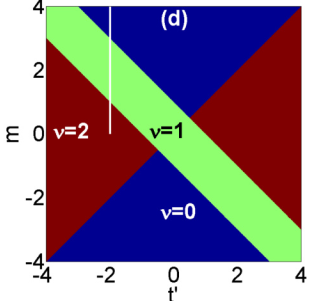
\includegraphics[width=35mm]{bdit1}
}}\hspace{0mm}

\makebox[0pt]{
\subfloat[$t = 1,t'=1$, \, $\kappa =\kappa'=0$]{
  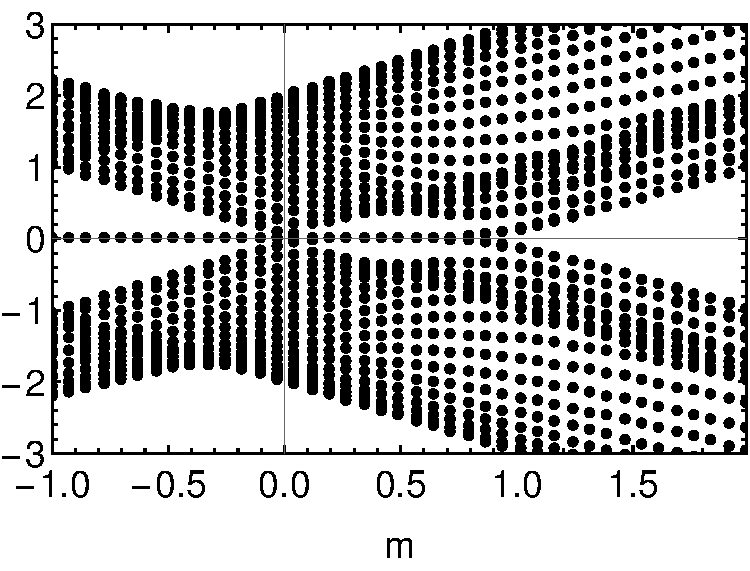
\includegraphics[width=35mm]{1_b.pdf}
}
\subfloat[$t=1,t'=1$, $\kappa = 0.3, \kappa'=0$]{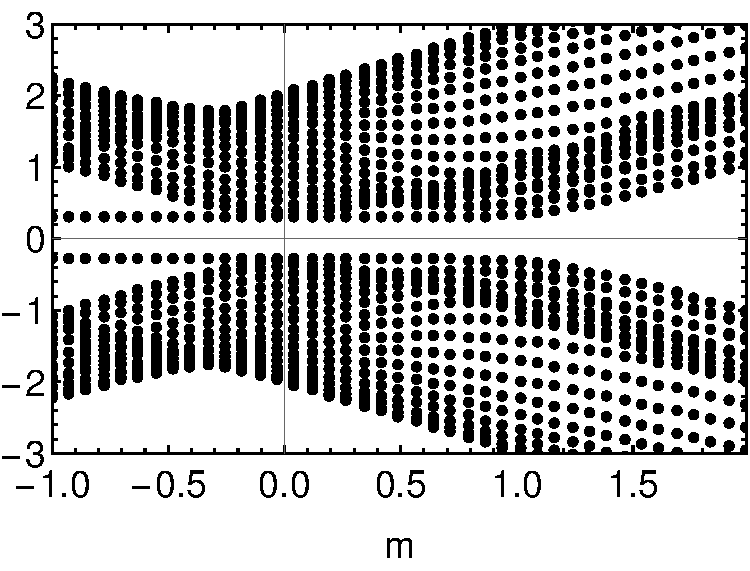
\includegraphics[width=35mm]{1_c.pdf}
}
}\hspace{0mm}

\makebox[0pt]{
\subfloat[$t = 1,t'=1$, $\kappa = 0,\kappa'=0.3$]{
  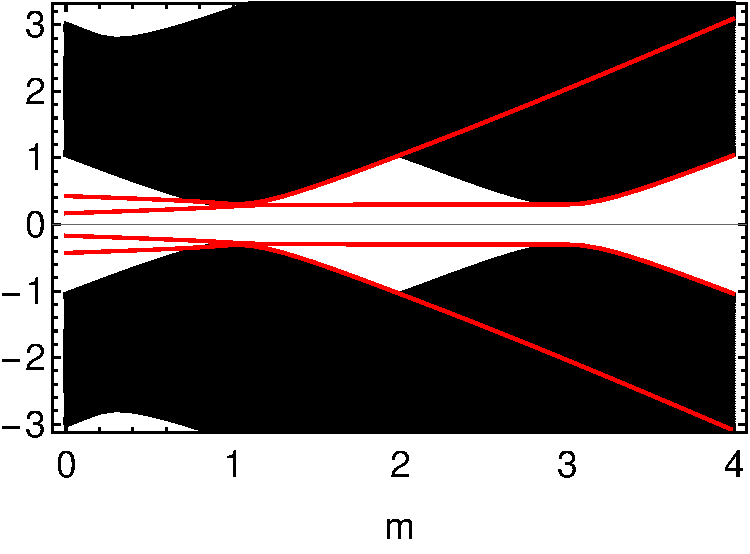
\includegraphics[width=35mm]{1_d.pdf}
}
\subfloat[$t=1,t'=1$, $\kappa = 0.3,\kappa'=0.3$]{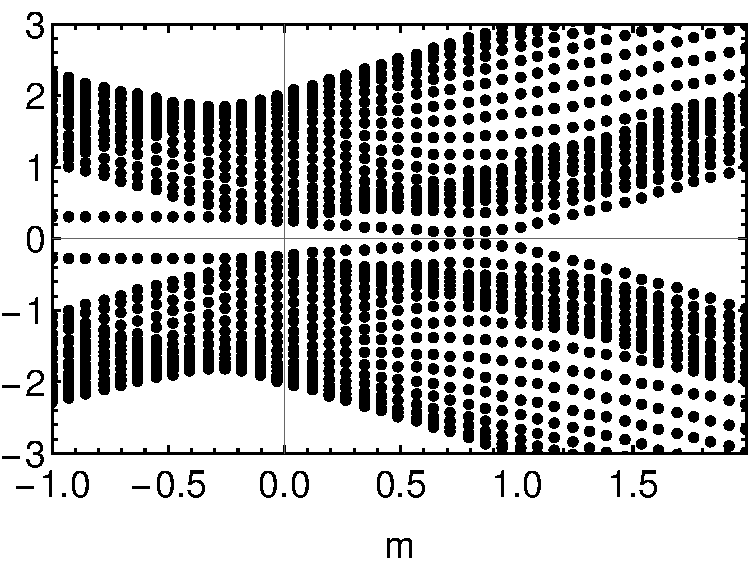
\includegraphics[width=35mm]{1_e.pdf}
}
}
\caption{Phase diagram for the system in the $BDI$ class showing the winding number of each region and surface energy spectrum for two different cuts in the phase diagram for different values of $\kappa,\kappa'$.}
\label{bdi_phase_diagram}
\end{figure}

\section{Geometric phase and Entanglement spectrum}
Consider a quadratic Hamiltonian in one dimension
\begin{equation}
\mathcal{H} = \sum_{ij,\alpha\beta} c_{i\alpha}^\dagger H_{ij,\alpha \beta}c_{j\beta}.
\end{equation}
We can obtain the single-particle eigenstates as
\begin{align*}
\sum_{j\beta}H_{ij,\alpha\beta} u^{p\mu}_{j\beta} = E_{p\mu} u_{i\alpha}^{p\mu},
\end{align*}
where $[U]_{j\beta,p\mu} = u^{p\mu}_{j\beta}$ is the unitary matrix that diagonalizes $H$. The polarization can be obtained as the many-body average of position operator, regularized for periodic boudnary conditions \cite{Resta1997}
\begin{align*}
\expval{X} = -\frac{L}{2\pi} \rm{ Im\, Ln }\bra{\Psi_0}e^{-i \frac{2\pi}{L}\hat{X}}\ket{\Psi_0},
\end{align*}
where $\ket{\Psi_0}$ is the many-body ground state and $\hat{X}$ is the sum of all the single-particle position operators.
Using that the ground state is a Slater determinant of the single-particle eigenstates, $\ket{u^{p\mu}}$, it can be rewritten as
\begin{align*}
\expval{\hat{X}} = -\frac{L}{2\pi} \rm{Im \, Ln}\, {\rm det} \, \tilde{S},
\end{align*}
where the matrix $\tilde{S}$ is obtained from another matrix S with elements
\begin{equation}
S_{p\mu,q\nu} = \sum_{j\alpha}u^{p\mu\, \ast}_{j \alpha} e^{-i\frac{2\pi}{L}j}u^{q\nu}_{j \alpha}
\end{equation}
by restricting it to the space of occupied single-particle states. The geometric phase can now be obtained as
\begin{equation}
\gamma = \expval{\hat{X}}\frac{2\pi}{L} + \frac{1}{2}
\end{equation}
\carlos{There is an extra 1/2 factor compared to Kivelson's formula which I don't know where it is coming from.}
The correlation function in position space is given by
\begin{align*}
C_{ij}^{\alpha \beta} = \expval{c_{i\alpha}^\dagger c_{j\beta}}.
\end{align*}
In terms of the fermions that diagonalize the Hamiltonian, 
\begin{align*}
& \gamma_{i\alpha} = \sum_{j\beta}u_{j\beta}^{i\alpha \, \ast} c_{j\beta} \\
& c_{i\alpha} = \sum_{j\beta} u^{j\beta}_{i\alpha} \gamma_{j\beta}
\end{align*}
we have
\begin{align*}
C_{ij}^{\alpha \beta} =& \sum_{pq,\mu\nu} u^{q\nu }_{j\beta} u^{p\mu \, \ast}_{i\alpha} \expval{\gamma^\dagger_{p\mu} \gamma_{q\nu} } \\
=&  \sum_{p\mu} u^{p\mu }_{j\beta} u^{p\mu \, \ast}_{i\alpha} \expval{\gamma^\dagger_{p\mu} \gamma_{p\mu} } \\
=&  \sum_{p\mu} u^{p\mu }_{j\beta} u^{p\mu \, \ast}_{i\alpha} [1-{\rm sign}(E_{p\mu})]/2.
\end{align*}
The first term is simply a kronecker delta between both sets of indeces. The second term can be rewritten as
\begin{align*}
UD(\abs{D})^{-1}U^\dagger =& UD(D^2)^{-1/2}U^\dagger \\
=& U D U^\dagger (U D^2 U^\dagger)^{-1/2} \\
=& H(H^2)^{-1/2},
\end{align*}
where $D$ is the diagonal Hamiltonian, $H=UDU^\dagger$. Finally the correlation function can be obtained in position space as
\begin{align*}
C_{ij}^{\alpha \beta} =& \frac{1}{2}\left[I - H/ (H^2)^{-1/2} \right]_{ij, \alpha \beta}
\end{align*}
The entanglement spectrum (ES) is then obtained as the spectrum of the subsystem correlation function obtained after bisecting the system into two equal parts. 

In the ES we can differentiate between two types of eigenvalues, which we denote by $\xi$. The ones at $\xi_b = 0,1$ correspond to bulk states while for the ones in between, $0<\xi_{l,r}<1$, we find their correspondent eigenstate localized in either the left, $\xi_l$, or right, $\xi_r$, virtual edge \carlos{Cite Peschel}. 

\section{Homogeneous system}

For symmetry-protected topological systems in one dimension there is a well-known relation between ES and the geometric phase. The geometric phase, which is quantized, is zero whenever there is an even number per edge of eigenvalues at $\xi = 1/2$, and $\pi$ when the number is odd. Beyond symmetry protected systems there have been observations, in simple systems with one edge-mode per edge, of similarities between the midgap eigenvalue of the entanglement spectrum and the geometric phase \cite{Ryu2006,Huang2012,Huang2012-2}, which in the case of the fully dimerized model becomes an exact identity \cite{Ryu2006}. 

Consider the combination of all eigenvalues localized in one of the edges modulo one,
\begin{equation}
\chi = \sum_{i \in r} \xi_i \quad {\rm mod} \quad 1. 
\end{equation}
As we will show below, one can find the geometric phase in the thermodynamic limit as
\begin{equation}
\lim_{L \rightarrow \infty}\gamma/2\pi =\lim_{L \rightarrow \infty} \chi.
\label{mainl}
\end{equation}
In the examples studied in references \cite{Ryu2006,Huang2012,Huang2012-2} the main contribution comes from one midgap state, while the rest of the edge states sit close to the bulk bands and therefore give a small contribution, which explains why the relation between the midgap eigenvalue and the geometric phase was almost an identity and why it breaks as we go deep into the trivial state. Alternatively, using that the entanglement spectrum is particle-hole symmetric for homogeneous systems we can express $\chi$ as
\begin{equation*}
\chi = \frac{1}{2} \left( \sum_{i\in r}\xi_i-\sum_{i\in l}\xi_i \pm \sum_{i\in b}\xi_i  + N_A \right) \quad {\rm mod} \quad 1,
\end{equation*}
where $N_A$ is the total number of electrons in subsystem A  in the ground state and the sign on the bulk term is irrelevant since $-1/2 \, {\rm mod} \, 1 = 1/2 \, {\rm mod} \, 1$. This form is preferable when doing numerics because due to finite size effects the bulk modes can acquire a finite eigenvalue and therefore in general it is difficult to classify between bulk and edge modes. \carlos{There is also the issue edge-modes and bulk-modes mixing in the inhomogenous case, introduce later?} In practice we diagonalize $C_A + \lambda C_A\hat{X}C_A$, where $\hat{X}$ is the position operator and $\lambda$ is a small parameter. The second term ensures that the originally degerate bulk states are also localized, so we can divide all eigenvalues in right and left sectors and assign the charges $1/2$ and $-1/2$, respectively. In Fig.\ref{bdi20} we show for several cases how Eq. \ref{mainl} holds up to finite size errors. $\chi$ is equivalent to the trace of the ES of a semi-infinite chain, but one can extract the information from the ES of a ring in the thermodynamic limit by looking at the localization structure of the eigenstates, only looking at the spectrum is not enough. 

One drastic example of this can be seen in figure \ref{old} , where two ES that look almost identical result in a very different geometric phase. 

\begin{figure}[h!]
\centering
\makebox[0pt]{
\subfloat[$t = 0, t' = 2, \kappa = 10^{-5}$]{
  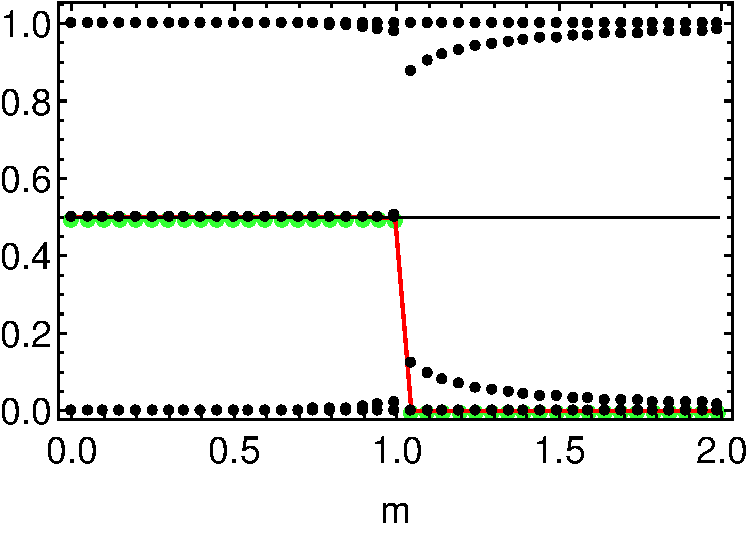
\includegraphics[width=35mm]{2_a.pdf}
}
\subfloat[$t = 0, t' = 2, \kappa = 0.3$]{
  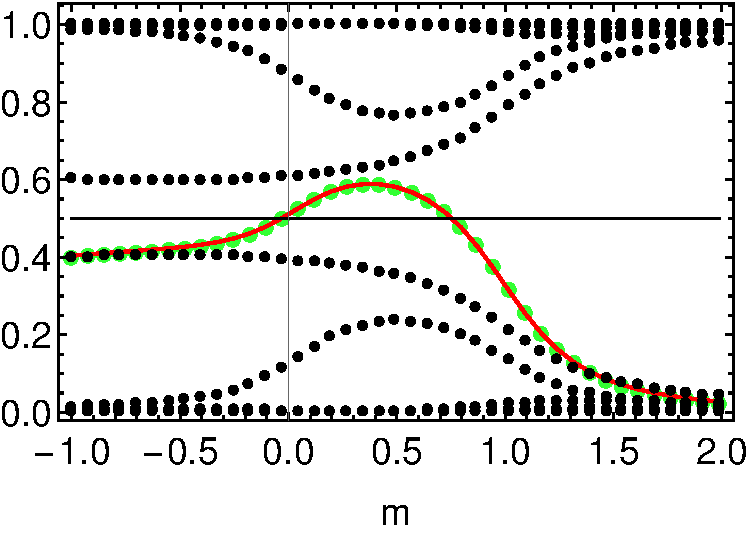
\includegraphics[width=35mm]{2_b.pdf}
}
}\hspace{0mm}

\makebox[0pt]{
\subfloat[$t = 0, t' = 2, \kappa = 10^{-5}$]{
  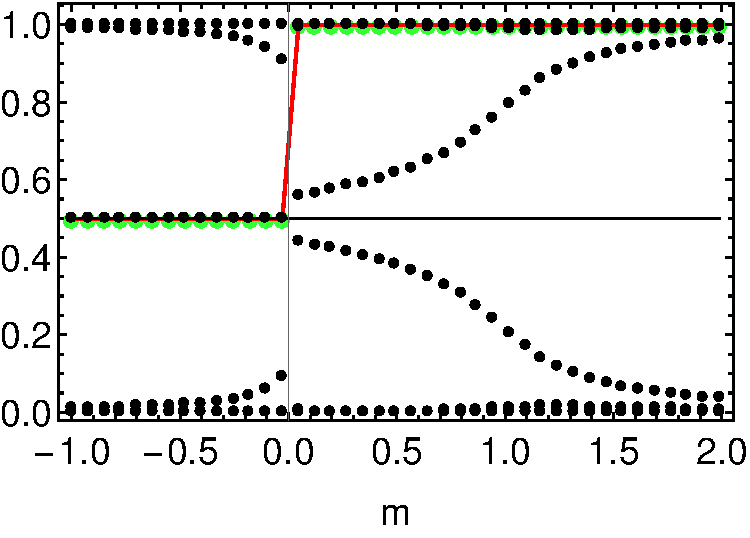
\includegraphics[width=35mm]{2_c.pdf}
}
\subfloat[$t = 0, t' = 2, \kappa = 0.3$]{
  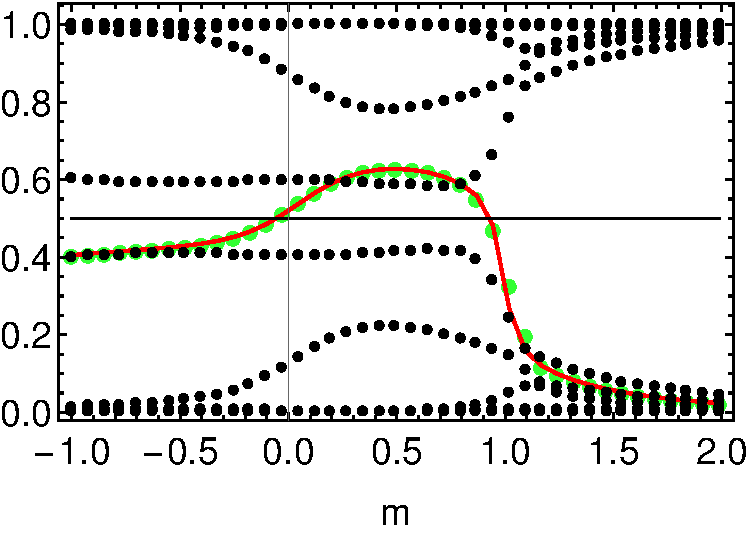
\includegraphics[width=35mm]{2_d.pdf}
}
}
\caption{fill. }
\label{bdi20}
\end{figure}
\begin{figure}[h!]
\centering
\makebox[0pt]{
\subfloat[$t = 0, t' = 2, \kappa = 10^{-5}$]{
  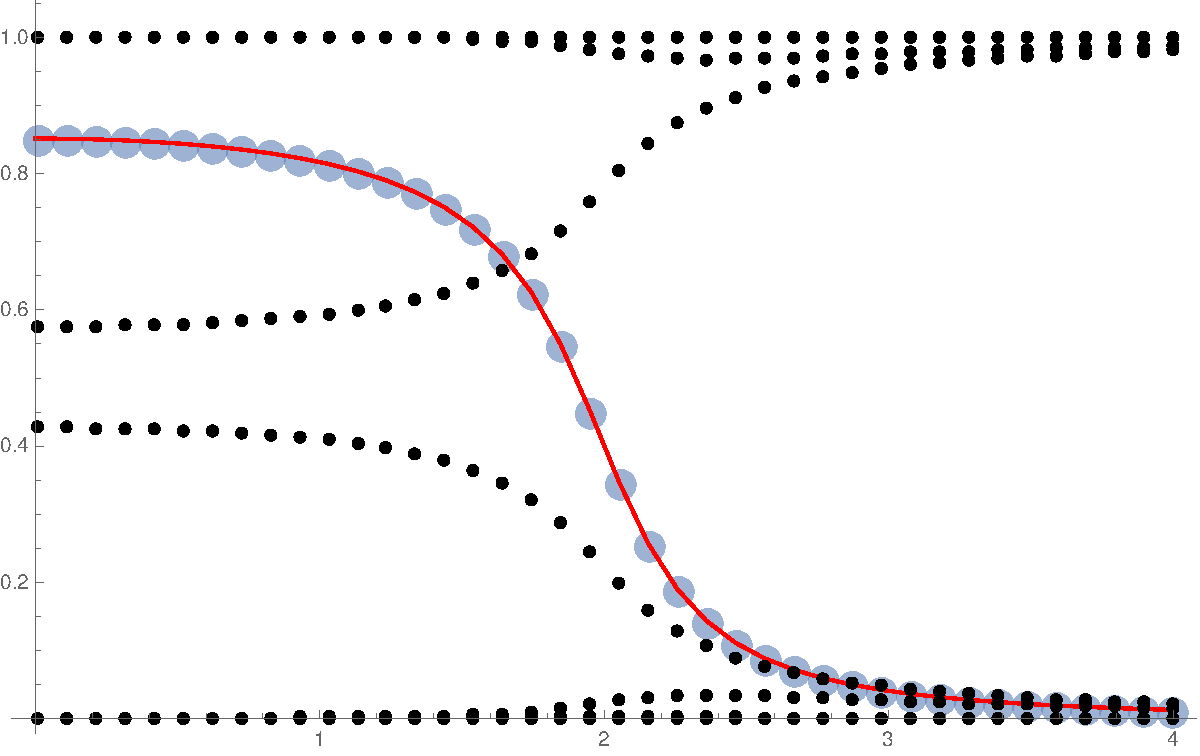
\includegraphics[width=35mm]{a20.pdf}
}
\subfloat[$t = 0, t' = 2, \kappa = 0.3$]{
  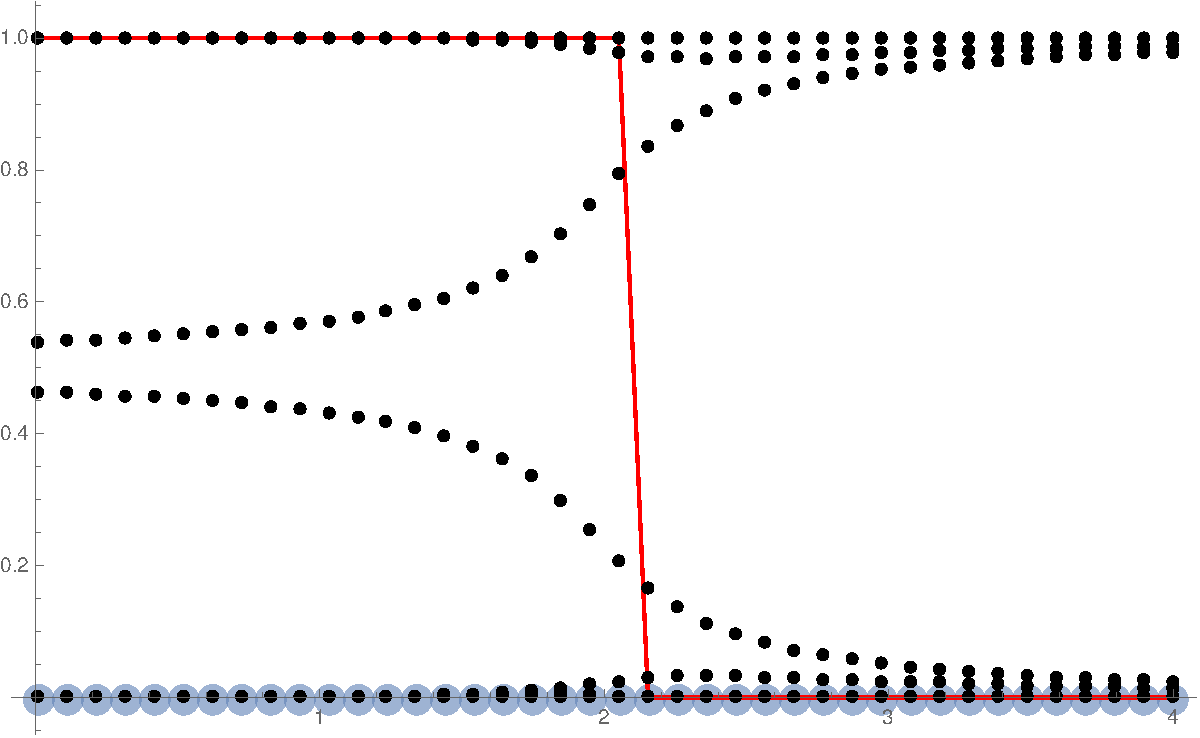
\includegraphics[width=35mm]{d20.pdf}
}
}
\caption{Old plot, do I keep it? }
\label{old}
\end{figure}

This relation between the geometric phase and the entanglement spectrum is a consequence of an identity between the geometric phase and the many-body entanglement spectrum previously found for infinite chains \cite{Zaletel2014}. In Appendix A (\carlos{I have to take a look at it again}) we modified this derivation to account for the periodic boundary conditions we use and show how their result reduces to Eq. \ref{mainl} when expressing it in terms of the ES.


\begin{figure}[h]
\centering
\makebox[0pt]{
\subfloat[$t = 0, t' = 2, \kappa = 0.3$]{
  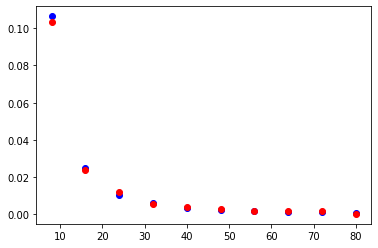
\includegraphics[width=65mm]{scaling_cut_disavg.png}
}
}
\caption{}
\label{disorder}
\end{figure}

\section{Inhomogeneous systems}

In reference \cite{Zaletel2014} translational invariance was used to derive Eq. \ref{zaletel} in Appendix A. Say we break translational invariance by adding weak disorder to the system. This will modify slightly the entanglement spectrum but not the charge assignment. Without translational invariance the entanglement spectrum will depend on where is the cut placed on the ring, even though the ground state, and therefore the geometric phase, will not. One thing one could do to get rid of the cut-dependence is to perform an average over all the spatial cuts of expression \ref{mainl}. Defining now the cut-dependent $\chi$ as 
\begin{equation*}
\chi_s = \frac{1}{2} \left( \sum_{i\in r}\xi^s_i-\sum_{i\in l}\xi^s_i \pm \sum_{i\in b}\xi^s_i  + N_A \right) \quad,
\end{equation*}
for a cut in positions $s$ and $s+L/2$. We can write
\begin{equation}
\gamma = \expval{\chi_s}_{\rm cuts} \, {\rm mod}\, 1.
\label{gphase_ih_mod}
\end{equation}
However this expression is not practical. In order for the bulk contribution to vanish with the modulo $1$ it has to be constant for different cuts. Last section we divided the bulk modes in right and left, but now we encounter the problem that their localization changes with the cut, so that there is the possibility that one bulk mode around $1/2$ changes its charge, leading to a wrong result. To get around this problem we can get rid of the bulk contribution before averaging,
\begin{equation}
\gamma = \expval{\chi_s \, {\rm mod}\, 1}_s \, {\rm mod}\, 1,
\label{gphase_ih_modmod}
\end{equation}
however the average of a circular quantity is not well defined. We will explain how one can perform the cut-average for different cases so that one can recover expression \ref{gphase_ih_mod} from expression \ref{gphase_ih_modmod}.

For the case when the width of $\chi_s$ is lower than one, there is a range of values $[x,x+1]$ where $\chi_s$ does not cross $0,1$, and averaging over this range makes sure than once we take the second modulo $1$ all the different possible results for the cut-average are reduced to a single one. The shortcomings of expression \ref{modmod} will be discussed later, but to show that this cut-average is correct we will consider now a system in the topological phase to which we add weak disorder, so one can then take the cut-average around $[0,1]$. In Fig.\ref{disorder} we show $1 - \expval{\chi_s \, {\rm mod}\, 1}_s \, {\rm mod}\, 1 /\gamma$ in red for different system sizes. In blue we have shown the same difference using a disorder average. Both values match fairly well and they seem to vanish in the thermodynamic limit, scaling as $O(L^{-2})$. The fact that different disorder configurations match so well points to a systematic finite-size error in the way we calculate either the ES or the geometric phase that is system-independent. From this result one could think that the cut-average is some sort of disorder average. The implication however goes in the opposite direction. If the cut-average is assumed to be correct, that implies that in the thermodynamic limit we can group all the infinite different disorder configurations into an infinite set of $L$ configurations relating to different cuts of the same system, which average individually to the correct $\gamma_{\rm conf}$.

For stronger disorder one cannot be sure if $\chi_s$ crosses $0,1$ or not so this method cannot be applied but for continuous inhomogeneous perturbations one can follow $\chi_s$, so we can use expression \ref{modmod} even when the inhomogeneity is strong. In Fig.\ref{4} we show the results using a position dependent $\kappa$ parameter, shown in figure \ref{4}.a. In cases Fig.\ref{4}.b,c the width of $\chi_s$ is small so we can average taking the value ranges $[0,1]$ and $[-1/2,1/2]$ respectively and we see that the cut average matches the geometric phase perfectly. However for stronger perturbations, as shown in Fig.\ref{4}.d, one can have that the width of $\chi_s$ is bigger than 1 and there is no meaningful range of values one can average. Instead what one can do is to "double the periodicity of $\chi_s$" by adding or substracting $1$ each time it crosses $0,1$, taking the cut-average of and then take the modulo 1. 

\begin{figure}[h!]
\centering
\makebox[0pt]{
\subfloat[]{
  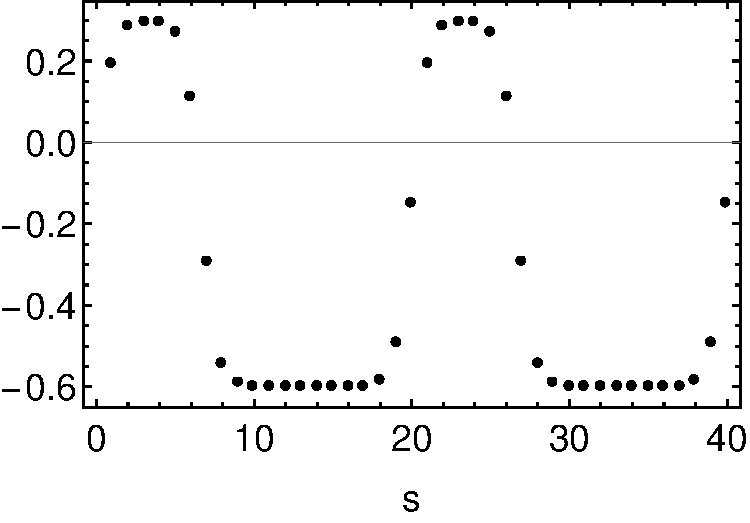
\includegraphics[width=40mm]{4_a.pdf}
}
\subfloat[]{
  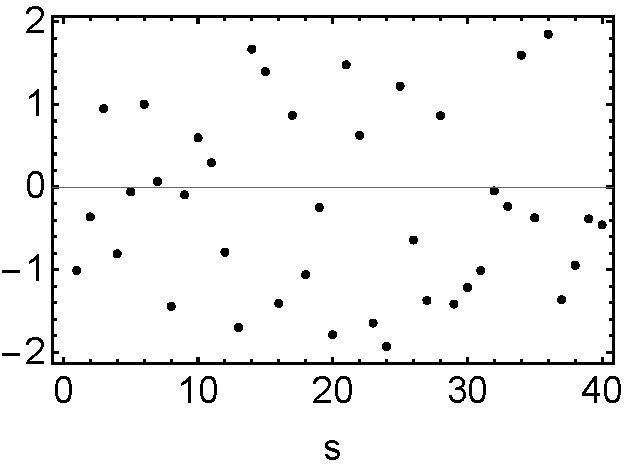
\includegraphics[width=40mm]{4_b.pdf}
}
}\hspace{0mm}

\makebox[0pt]{
\subfloat[]{
  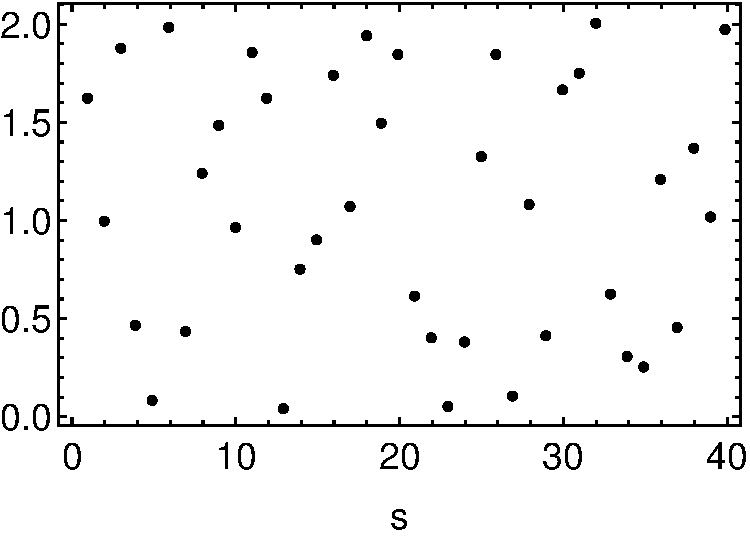
\includegraphics[width=40mm]{4_c.pdf}
}
\subfloat[]{
  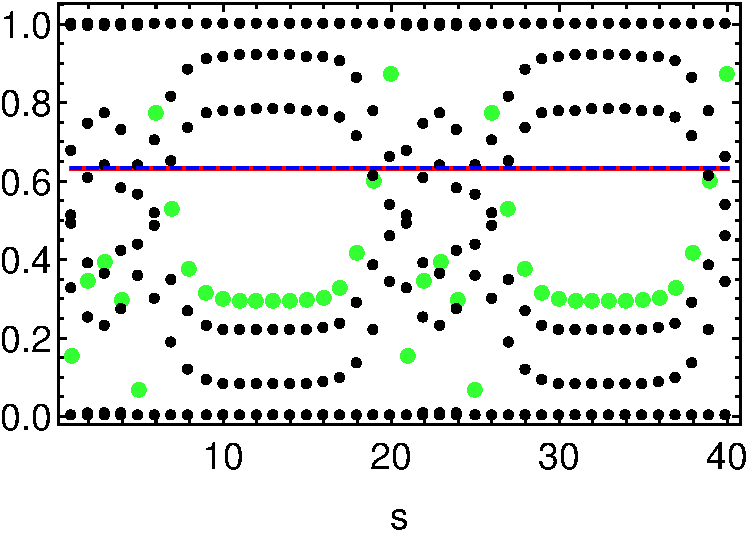
\includegraphics[width=40mm]{4_d.pdf}
}
}


\caption{ fill. put .5 line, also break the symmetry. with an envelope.}
\label{4}
\end{figure}

In Fig.\ref{4} we use a profile which is invariant for $x\rightarrow x+L/2$ because it enhances the effect of the nonhomogeneity, but this symmetry is not necesarry for anything we discuss here.

Another case where one can find a solution to the issue when cut-averaging is when the system is fully gapped, so that the ES doesn't have modes crossing $1/2$ for any cut. In this case one can make use of the particle-hole symmetry of the ES (If $\xi$ is an eigenvalue for a cut in $s$ then $1-\xi$ is an eigenvalue of the cut in $s+L/2$) and use only the lower half of the spectrum to build $\chi_s$ so that the bulk contribution vanishes enitrely. 
One can explot the fact that, even in the inhomogeneous case, the ES has a type of particle-hole symmetry. 

Another interesting point to note is that the two charge choices now leave to different $\chi_s$ since the particle-hole symmetry is no longer fulfilled for individual cuts. However both still lead to the same result because of the particle-hole time $L/2$ translation symmetry. Interestingly for the half-integer charge choice the quantity $\chi_s$ seems to be smaller, leading to fewer issues when averaging. 





\section{Superconducting systems}

The proof in Ref.\cite{Zaletel2014} also breaks down for superconducting systems. However, as we did for systems without translational invariance, one can extend expression \ref{mainl} for systems with pairing terms as well. Since one computes the geometric phase from the single-particle Bogoliubov-de Gennes Hamiltonian, we can obtain the correspondent entanglement spectrum and use expression \ref{mainl} to obtain the geometric phase. Take for example the kitaev chain, with the following Hamiltonian
\begin{align*}
H =& -\mu \sum_{i} c_i^\dagger c_i - t \sum_{i}\left( c_{i+1}^\dagger c_i + {\rm h.c.}\right) \\
&+  \sum_{i}\left( \Delta c_{i} c_{i+1} + {\rm h.c.}\right).
\end{align*}
Using the spinor $\phi_i^\dagger = (c_i^\dagger, c_i)$, we can rewrite the Hamiltonian as
\begin{align*}
&H = \frac{1}{2}\sum_i \phi^\dagger_i H_{BdG,ij} \phi_j,\\
&H_{BdG,ij} = -\mu \tau_z \delta_{ij} - (t \tau_z + i\Delta \tau_y )\delta_{i,j+1}- (t \tau_z - i\Delta \tau_y)\delta_{i,j-1}.
\end{align*}
Note that by taking $t' = \kappa = \kappa = 0$ in the BDI model, Eq. \ref{bdi_model}, we obtain
\begin{align*}
H_{ij} =& m \sigma_x\delta_{ij} + \frac{1}{2} t \left[(\sigma_x + i \sigma_y)\delta_{i,j+1} + (\sigma_x - i \sigma_y) \delta_{i,j-1} \right],
\end{align*}
which is just the Bogoliubov-de Gennes Hamiltonian of the Kitaev chain by rotating $x$ into $z$ and identifying $\mu = -m, t_{\rm Kit} = -t_{BDI}/2, \Delta = -t_{BDI}/2 $. From Fig.\ref{bdi_phase_diagram} we see that the $BDI$ model transitions from $\nu = 1$ to the trivial phase at $t=0, m=\pm t_{BDI}$, or alternatively, when $\mu = \pm 2 t_{Kit}$, which is the known result for the Kitaev chain. Therefore the results already shown for the BDI model studied here are also applicable to the Kitaev chain.  

\bibliography{references}	

	
\appendix

\section{Appendix A}
	
Consider a chain with periodic boundary conditions. A Schmidt decomposition for two bipartite cuts gives the ground state
\begin{equation}
\ket{\psi} = \sum_{p,q} \ket{p,q}_A s_p \ket{p,q}_B s_q,
\end{equation}
where we assume that the size of each subsystem is big enough so that the cuts can be considered independent of each other. We can now take subsystem B and glue its ends together to obtain the ground state of a ring with a single cut. If we include a flux threading inside the ring we obtain
\begin{equation}
\ket{\psi^\phi} = \sum_p s_p \ket{p,p}_B e^{i\phi Q_p},
\end{equation}
The many-body states $\ket{p,p}_B$ can be built by occupying the different ES eigenstates and are therefore characterized by a set of occupying numbers $\{n\}_p$. The many-body entanglement spectrum can also be expressed in terms of the single-particle one \cite{Alexandrinata2011} as
\begin{align}
s_p^2 =& \prod_{i \in {\rm occ}} \xi_i \prod_{i \in {\rm empty}}(1-\xi_i) \\
=& \prod_i (1-\xi_i)\left(\frac{\xi_i}{1-\xi_i} \right)^{n_i}
\end{align}
And the charge can be assigned so that $Q_p = \sum_{\alpha = b,l,r} q_\alpha\sum_{i \in \alpha} n_i$ with the constrain that $q_r,\pm q_b = q_l-1$ \textcolor{red}{Why?}. As the main result of \cite{Zaletel2014} the geometric phase is then found to be
\begin{align}
e^{i\gamma} = e^{2\pi i \sum_p s_p^2 Q_p}  \bra{\psi^0}\ket{\psi^{2\pi}},
\label{zaletel}
\end{align}
where the monodromy is given by
\begin{align}
\bra{\psi^0}\ket{\psi^{2\pi}} =& \sum_p s_p^2 e^{2\pi i Q_p}.
\end{align}
Consider the exponential term
\begin{align*}
e^{2\pi i (q_L N^p_l + (1-q_l)(N^p_r+N^p_b))} =& e^{2\pi i (q_l N^p_l + (1-q_l)(N-N^p_l))} \\
=& e^{4\pi i q_l N^p_l}e^{2 \pi i (N-N^p_l)}e^{-2\pi i q_l N },
\end{align*}
where $N^p_\alpha = \sum_{i \in \alpha} n_i$ and the total number of electrons, $N = \sum_{\alpha = b,l,r} N^p_\alpha$, is independent of $p$. We will consider two natural choices, $q_l = 1,1/2$, for which we have
\begin{align}
\bra{\psi^0}\ket{\psi^{2\pi}} =& 
\begin{cases}
1 & \text{for} \quad q_l = 1 \\
e^{N\pi i} & \text{for} \quad q_l = 1/2,
\end{cases}
\end{align}
where we used that $\sum_p s_p^2 = 1$. The change in the monodromy between both choices is accompanied by a change in the exponential term in Eq.\ref{zaletel}, so that both charge choices are equivalent.

Expressing the contribution of the many-body entanglement spectrum to the geometric phase in terms of the ES, we have
\begin{align*}
\gamma' = 2\pi \sum_{n_i = 0,1} \left(\sum_{i } n_i q_i\right) \left(\prod_m (1- \xi_m)\left(\frac{\xi_m}{1-\xi_m} \right)^{n_m} \right) ,
\end{align*} 
Consider now its derivative with respect to a particular entanglement eigenvalue
\begin{align}
\frac{1}{2\pi}\frac{\partial \gamma'}{\partial \xi_p} =& \sum_{\{n_k\}=0,1}\left(\sum_{i } n_i q_i\right)\frac{n_p - \xi_p}{\xi_p^{1-n_p}(1-\xi_p)^{n_p}}\\
&\times \left(\prod_{m\neq p} (1- \xi_m)\left(\frac{\xi_m}{1-\xi_m} \right)^{n_m} \right)
\end{align}
where
\begin{equation}
 \frac{n_p - \xi_p}{\xi_p^{1-n_p}(1-\xi_p)^{n_p}} = 
  \begin{cases}
    -1, & \text{for } n_p=0 \\
    1, & \text{for } n_p = 1 \\
  \end{cases}	
\end{equation}
Therefore we have
\begin{align*}
\frac{1}{2\pi}\frac{\partial \gamma'}{\partial \xi_p} =& -\sum_{\substack{\{n_{k\neq p}\}=0,1 \\ n_p = 0}}\left(\sum_{i \neq p} n_i q_i\right)\prod_{m\neq p} (1-\xi_m)\left( \frac{\xi_m}{1-\xi_m} \right)^{n_m} \\
&+ \sum_{\substack{\{n_{k\neq p}\}=0,1 \\ n_p = 1}}\left(\sum_{i \neq p} n_i q_i +q_p\right) \prod_{m\neq p} (1-\xi_m)\left( \frac{\xi_m}{1-\xi_m} \right)^{n_m} \\
=&q_p\sum_{\{n_{k\neq p}\}=0,1} \prod_{k\neq p} (1-\xi_k)\left( \frac{\xi_k}{1-\xi_k} \right)^{n_k} \\
\end{align*}
Expand now the sum  for another occupation number $n_{p'} = 0,1$ 
\begin{align*}
\frac{1}{2\pi}\frac{\partial \gamma'}{\partial \xi_p} =& q_p\sum_{\substack{n_{k \neq p \neq p'}=0,1\\ n_{p'}= 0}} (1-\xi_{p'})\prod_{k\neq p,p'} (1-\xi_k)\left( \frac{\xi_k}{1-\xi_k} \right)^{n_k} \\
&+ q_p\sum_{\substack{n_{k \neq p \neq p'}=0,1\\ n_{p'}= 1}} \xi_{p'}\prod_{k\neq p,p'} (1-\xi_k)\left( \frac{\xi_k}{1-\xi_k} \right)^{n_k} \\
 &=q_p\sum_{\substack{n_{k \neq p \neq p'}=0,1}} \prod_{k\neq p,p'} (1-\xi_k)\left( \frac{\xi_k}{1-\xi_k} \right)^{n_k} 
\end{align*}
doing this for the rest of the occupation numbers we obtain 
\begin{equation}
\frac{1}{2\pi}\frac{\partial \gamma'}{\partial \xi_p} = q_p,
\end{equation}
so that 
\begin{align*}
\gamma =& \gamma' - i\log(\bra{\psi^0}\ket{\psi^{2\pi}})\\
=& \sum_{i}q_i \xi_i - i\log(\bra{\psi^0}\ket{\psi^{2\pi}})\\
\end{align*}
and we have recovered equation \ref{mainl}. 

\end{document}